\documentclass[a4paper]{article}
\usepackage[top=1in, bottom=1in, left=0.8in, right=0.8in]{geometry}
\usepackage{amsmath}
\usepackage{graphicx}
\usepackage{subfig}
\usepackage{wrapfig}
\usepackage{float}
\begin{document}


{\centering\huge Digital Visual Effects Project 2 Report\par}
{\centering b03901057 Chin-Cheng Chan, b03901089 Tzu-Peng Wang\par}
\noindent\makebox[\linewidth]{\rule{16cm}{1pt}} \\

In this project, we have implemented an image-stitching program in C++ with OpenCV
for image processing. The details of the implementation along with the results and
discussions are presented in this report.

\section{Project Overview}
Throughout this project, we have chosen the cylindrical projection model due to
its simplicity. However, this simple model also gives rise to a bunch of limitations
on the problems we can handle. Under this model, we can only stitch sequences of
images that are shot with a carefully calibrated camera, such as the "parrington"
dataset. Despite the limitations, some of our photos are taken with a handheld
iPhone, and we can still produce panorama with great quality through our program.

The entire process can be separated into five major components: image warping,
feature extraction, feature matching, image matching, and blending.

\section{Image Warping}
We implemented an inverse cylindrical warping method that takes the camera calibration
parameters (e.g. focal length) from other source, such as Autostitch, and then warp the
image using bilinear interpolation as the resampling method. Since these are all
introduced in class, we are not going to talk much about this part. Please refer
to our code for more implementation details.

Note that we taken the parameters from other software because our program lacks
the ability to optimize for the best camera parameters to match the images.

The following example demonstrates how warping helps aligning the images. (though
there still exists some slight misalignments after warping)

\begin{figure*}[h]
  \centering
  \subfloat[Without warping] {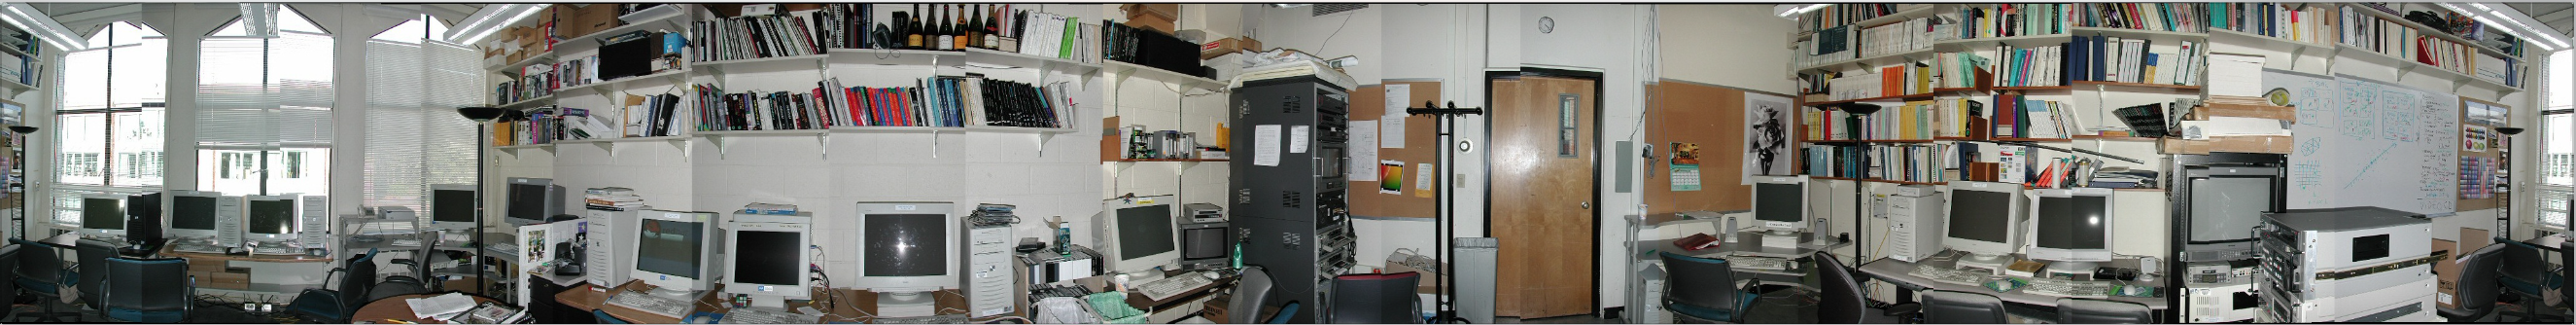
\includegraphics[width=\textwidth]{./figs/no-warp.png}}
  \vspace{0.2cm}
  \subfloat[With warping] {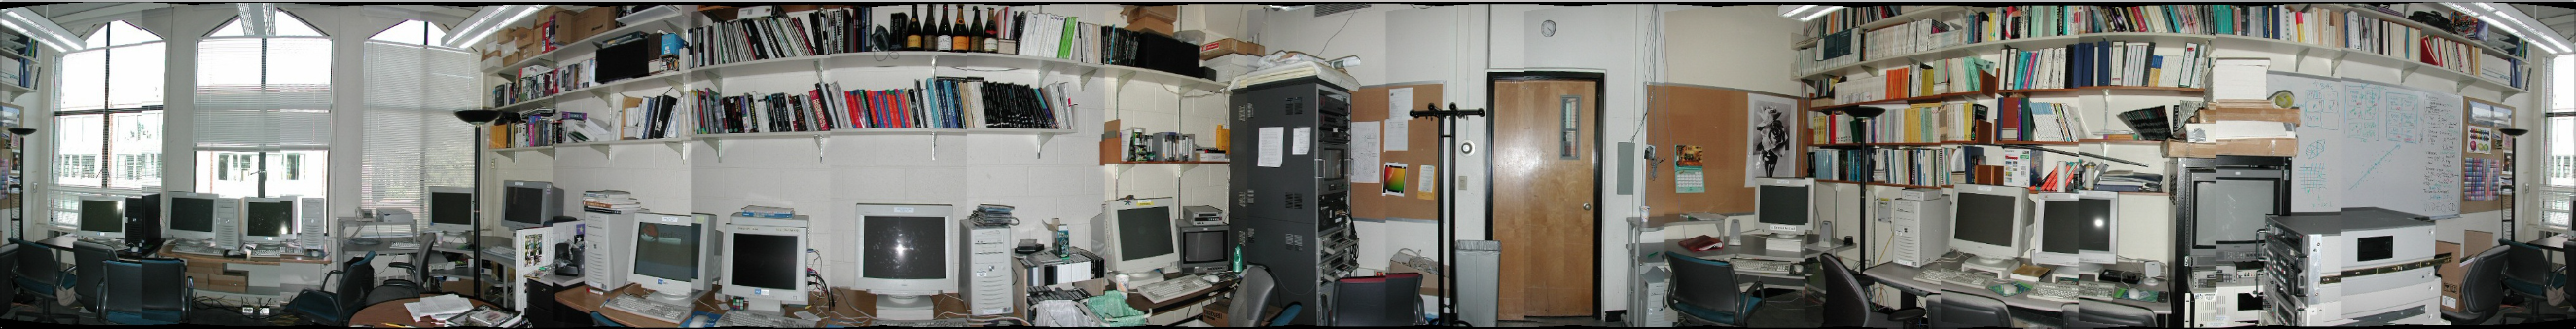
\includegraphics[width=\textwidth]{./figs/warp.png}}
  \caption{Comparison using the ``grail'' dataset. The images are directly stitched together.}
  \label{fig:warp}
\end{figure*}

\section{Feature Extraction}
The next step is feature extraction, and we choose to implement the MSOP \cite{brown2005multi} feature detector in this project because this feature detector is designed specifically for image matching and it balances the performance and the complexity.

\subsection{Algorithm description}

Our implementation and parameters basically follow the original paper. Nonetheless, the general procedure of our implementation is described below:
\begin{enumerate}
  \item Convert the input RGB image to gray scale and build an image pyramid for the gray scale image. The height of the pyramid (how many layers) is determined by the size of image such that the size of the smallest image of the pyramid is not smaller than 20\% of its original size.
  \item For each image in the pyramid, we compute the corner strength function, and use a threshold on the corner strength to select a few candidate interest points. Then, the positions of the candidate interest points are refined to sub-pixel level by fitting of quadratic function.
  \item After selecting candidate interest points for each image of the pyramid, we collect these candidate interest points and apply the adaptive non-maximum suppression to select the final set of interest points such that these points are evenly distributed throughout the image. The number of final interest points is set to $500$ in our project.
  \item Finally, we compute a descriptor for each interest point. We use the same descriptor as proposed in the original paper.
\end{enumerate}

\subsection{Adaptive Non-maximal Suppression}
One thing worth noting is our implementation of the ANMS process. At first glance,
this can be the bottleneck of the MSOP process due to its time complexity of $O(n^2)$
if implemented in a brute-force way, which can be really time-consuming once the
amount of interest points goes beyond $20000$ or so. The original paper introduced
another algorithm that first sorts all interest points by their strength and
then compute the maximum radius for a point by scanning through all points with
greater strength. Finally, we sort the points by the computed radius and select
the $500$ points with the largest radius.  This implementation, though avoiding
some unnecessary comparisons, still runs in $O(n^2)$.

Here, we improve the algorithm to run in $O(nlog^2n)$. The key observation is that
for each point, the problem to solve is in fact the nearest neighbor problem,
considering only the points with strength greater than it. So, we can use a kd-tree
with 2-dimensional data to solve the problem. Note that the kd-tree here should
support the insertion operation. So we looked up some implementations and made some
easy tweaks to let it support the operations we need. Anyway, to support fast insertion
involves rebuilding part of the tree and some amortized analysis. Please refer
to our source code for further implementation details.

With this data structure, we can see a significant speedup when there are tens of
thousands of interest points to consider.

\subsection{Results}
Some results of our feature detector are shown: \\
\begin{figure*}[h]
  \centering
  \subfloat[Without suppression] {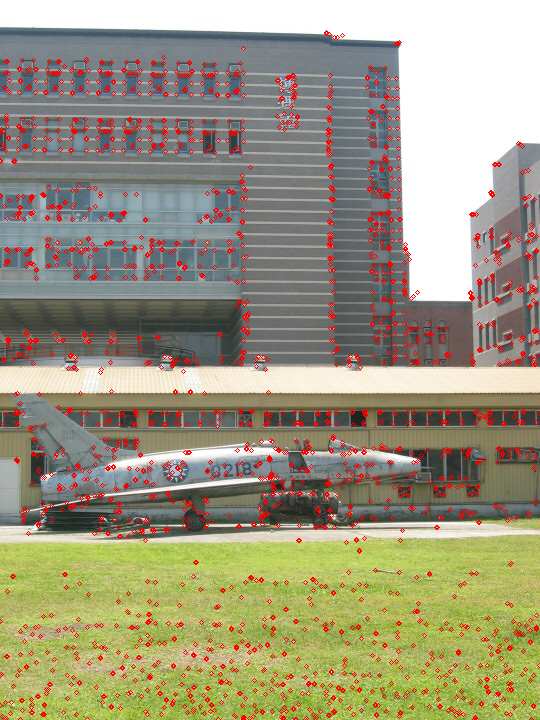
\includegraphics[width=0.3\textwidth]{./figs/all_corners.png}}
  \hspace{1.0cm}
  \subfloat[After suppression, r = 23.1] {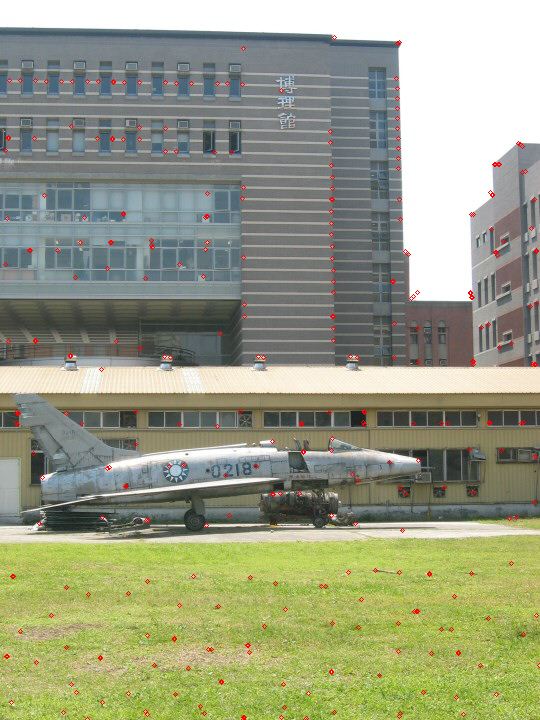
\includegraphics[width=0.3\textwidth]{./figs/corner_sup.png}}
  \caption{\textbf{Interest points detected from the ``csie'' dataset.} (a) Interest points without non-maximal suppression. (b) Interest points after non-maximal suppression. Red dots are detected interest points}
  \label{fig:csie}
\end{figure*}

The effect of the adaptive non-maximal suppression can be clearly seen in Fig. \ref{fig:csie}. Before suppression, we have a lot of unevenly distributed interest points. This phenomenon not only increases the computational cost, but also introduces redundant information because points that are close to each other are likely to generate similar descriptors. As a result, it is desirable to keep these points separated. It can be seen in Fig. \ref{fig:csie}(b) that after the suppression, points are much more evenly distributed. \\

Then we visualize the interest points extracted from each layer of the pyramid: \\
\begin{figure*}[h]
  \centering
  \subfloat[First layer. Full scale] {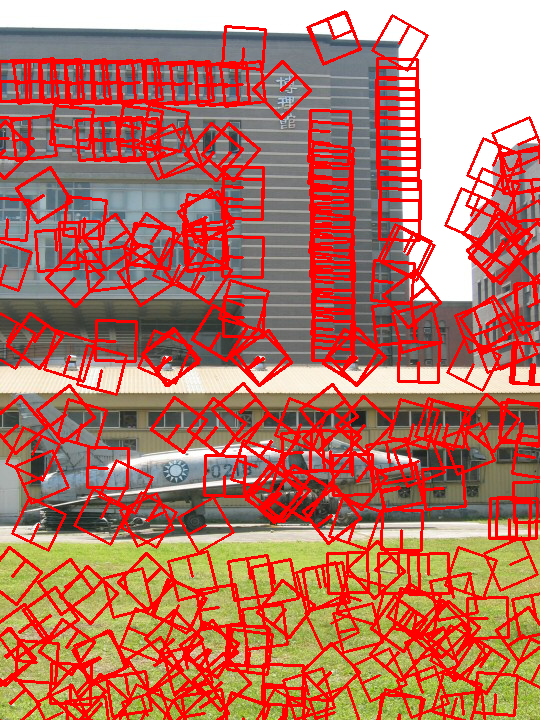
\includegraphics[width=0.3\textwidth]{./figs/lay_0.png}}
  \hfill
  \subfloat[Second layer. 0.5x] {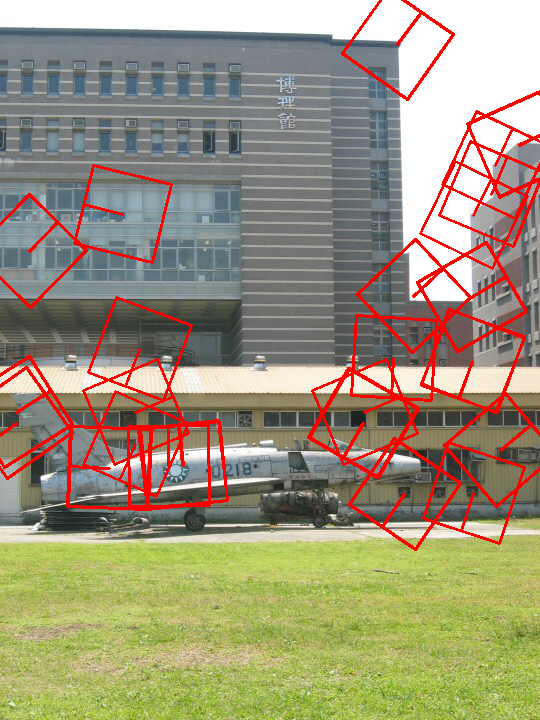
\includegraphics[width=0.3\textwidth]{./figs/lay_1.png}}
  \hfill
  \subfloat[Third layer. 0.25x] {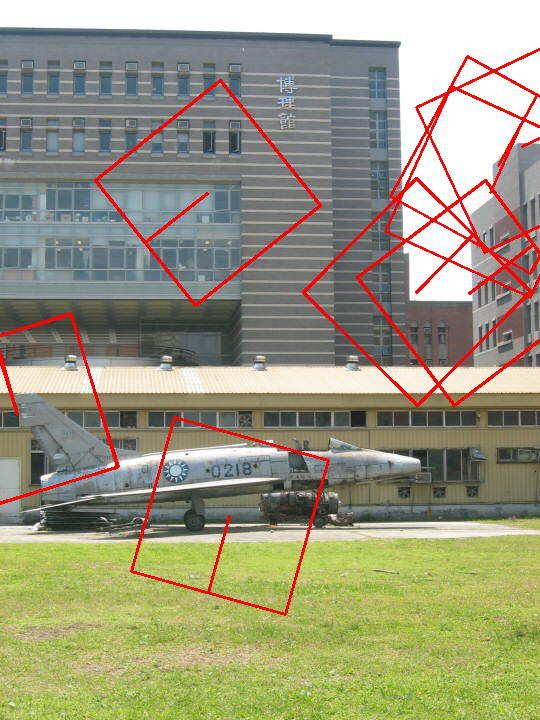
\includegraphics[width=0.3\textwidth]{./figs/lay_2.png}}
  \caption{\textbf{Interest points extracted from image with different scale}. (a) Original image (full scale). (b) Half size. (c) 1/4 size}
  \label{fig:three_scales}
\end{figure*}

It can be seen from Fig. \ref{fig:three_scales}(c) that the location of interest points are not very accurate. This is because the image from which these features are extracted is severely down-samples, so the these points may deviate from the true corners when their positions are up-sampled to the full scale for display.

\section{Feature Matching}
From the previous stage, we've computed a 64-dimensional data as the descriptor
of a feature point. Now for feature matching between two images, we implemented
two methods: exhaustive search and the kNN method.

\subsection{Exhaustive Search}
The exhaustive search method scans through all pairs of feature point between the
two images. For a pair of feature to match, two criteria must be satisfied:

\begin{enumerate}
  \item {\bf Must be close enough to each other.} Both feature points must be among
    one of the nearest point to each other. This is to eliminate the case where
    a feature point in fact doesn't match any point on the other image.
  \item {\bf Must be close enough on the y-axis.} This is a simple hueristic to
    eliminate as many outliers as possible since under the cylindrical projection
    model, two feature points with y-coordinates far from each other are very unlikely
    to be inliers.
\end{enumerate}

\subsection{FLANN}
As for the kNN method, we use the \texttt{flann} included in OpenCV to help do
the task of finding nearest neighbors. The same criteria described above must
also be satisfied in this case. This method is asymptotically more effiecient than
the exhaustive search method.

The following example demonstrates how the criteria are eliminating outliers and
also shows how features are matched. Including the two criteria significantly
increases the proportion of inliers.

\begin{figure*}[h]
  \centering
  \subfloat[No criteria is required] {\includegraphics[width=0.32\textwidth]{./figs/feat_match0.png}}
  \hfill
  \subfloat[Only the first criteria is required] {\includegraphics[width=0.32\textwidth]{./figs/feat_match1.png}}
  \hfill
  \subfloat[Both criteria are required] {\includegraphics[width=0.32\textwidth]{./figs/feat_match2.png}}
  \caption{\textbf{Feature matches between two images under different criteria settings}}
  \label{fig:featMatch}
\end{figure*}

\section{Image Matching}
After we match the feature points, we utilize the RANSAC algorithm along with
translational model to compute the best shift that aligns the two images. In our
program, we use $5$ sample points and $2000$ rounds to find the best fit.

As for global shift, we compute the accumulated shift of each image and save them
for the last stage, blending. At this point, we also handle the global y-directional
drift by splitting the drift uniformly to each image, the method introduced in class.

We use the ``parrington'' dataset below to demonstrate the result of image matching.

\begin{figure*}[h]
  \centering
  \subfloat[No drift correction] {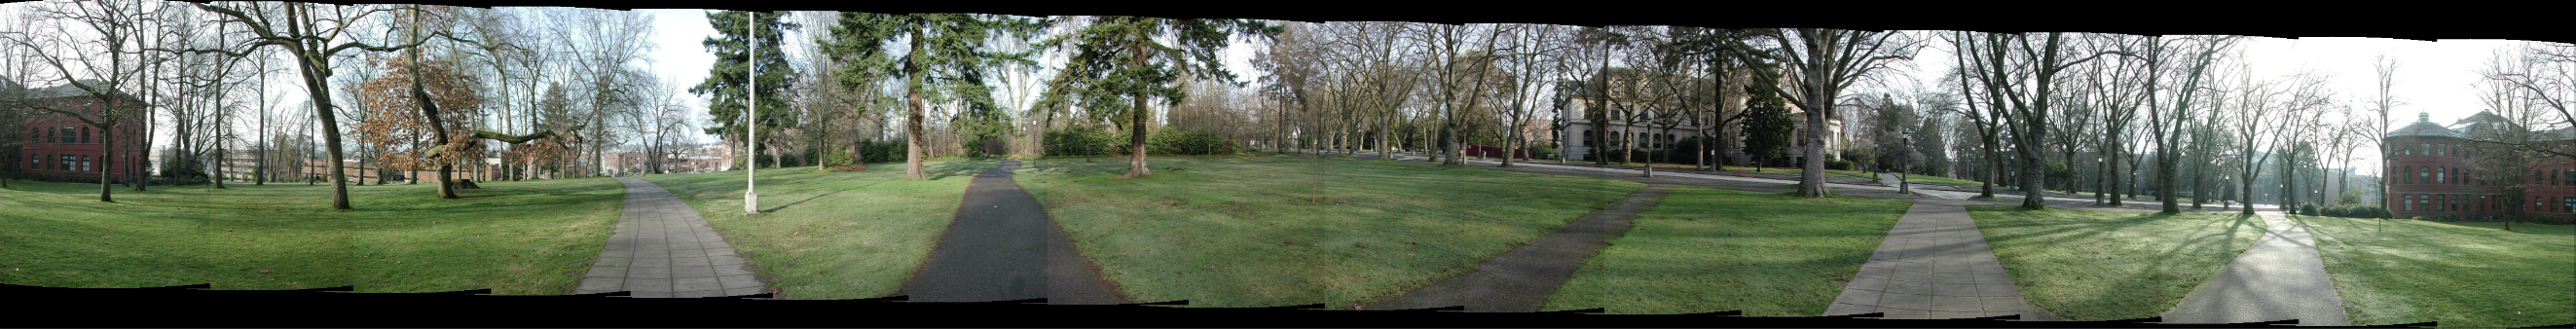
\includegraphics[width=\textwidth]{./figs/drift.png}}
  \hfill
  \subfloat[With drift correction] {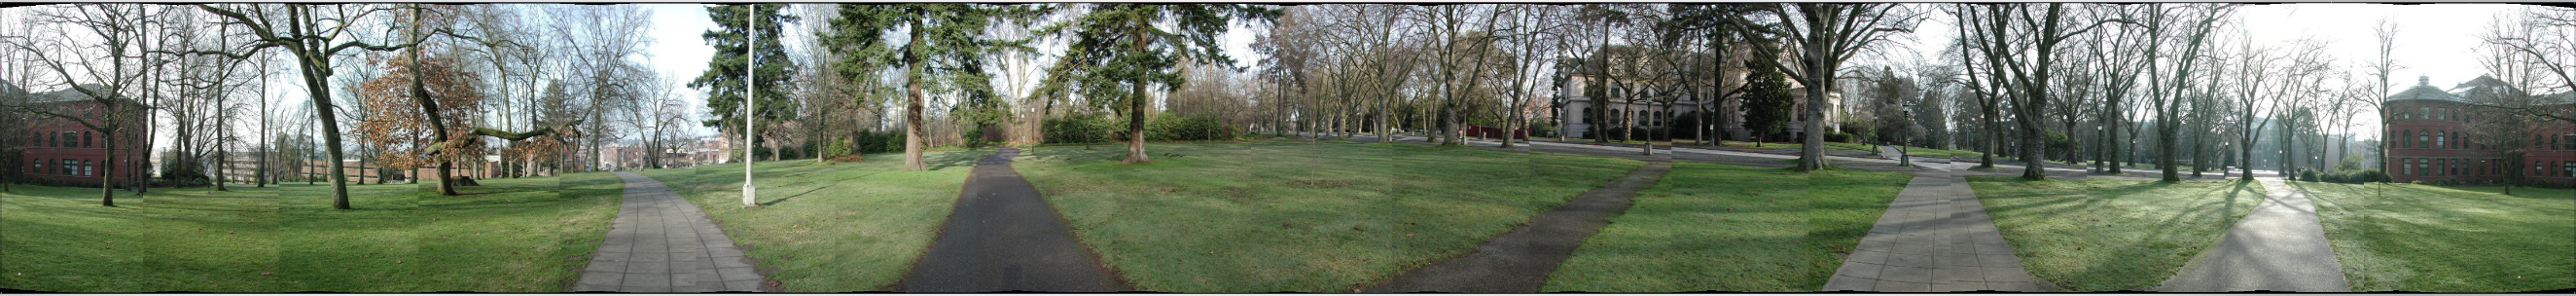
\includegraphics[width=\textwidth]{./figs/no-drift.png}}
  \caption{\textbf{Image Matching (direct blended)}}
  \label{fig:imageMatch}
\end{figure*}

\section{Blending}
The final step of creating awesome panorama is to blend the aligned images seamlessly.
We implemented three different blending methods: direct blending, alpha blending,
and poisson blending. We will analyze their pros and cons in this section.

\subsection{Direct Blending}
This is the easiest blending method. However, it only works well when the brightness
between images are consistent and the images are well aligned. Otherwise, it is
easy to spot the boundaries where images are concatenated together.

From the previous and the following artifacts using direct blending, it's easy
to tell that the blending is not seamless enough and often results in poor panorama.

\begin{figure*}[h]
  \centering
  \subfloat[Temple using direct blending] {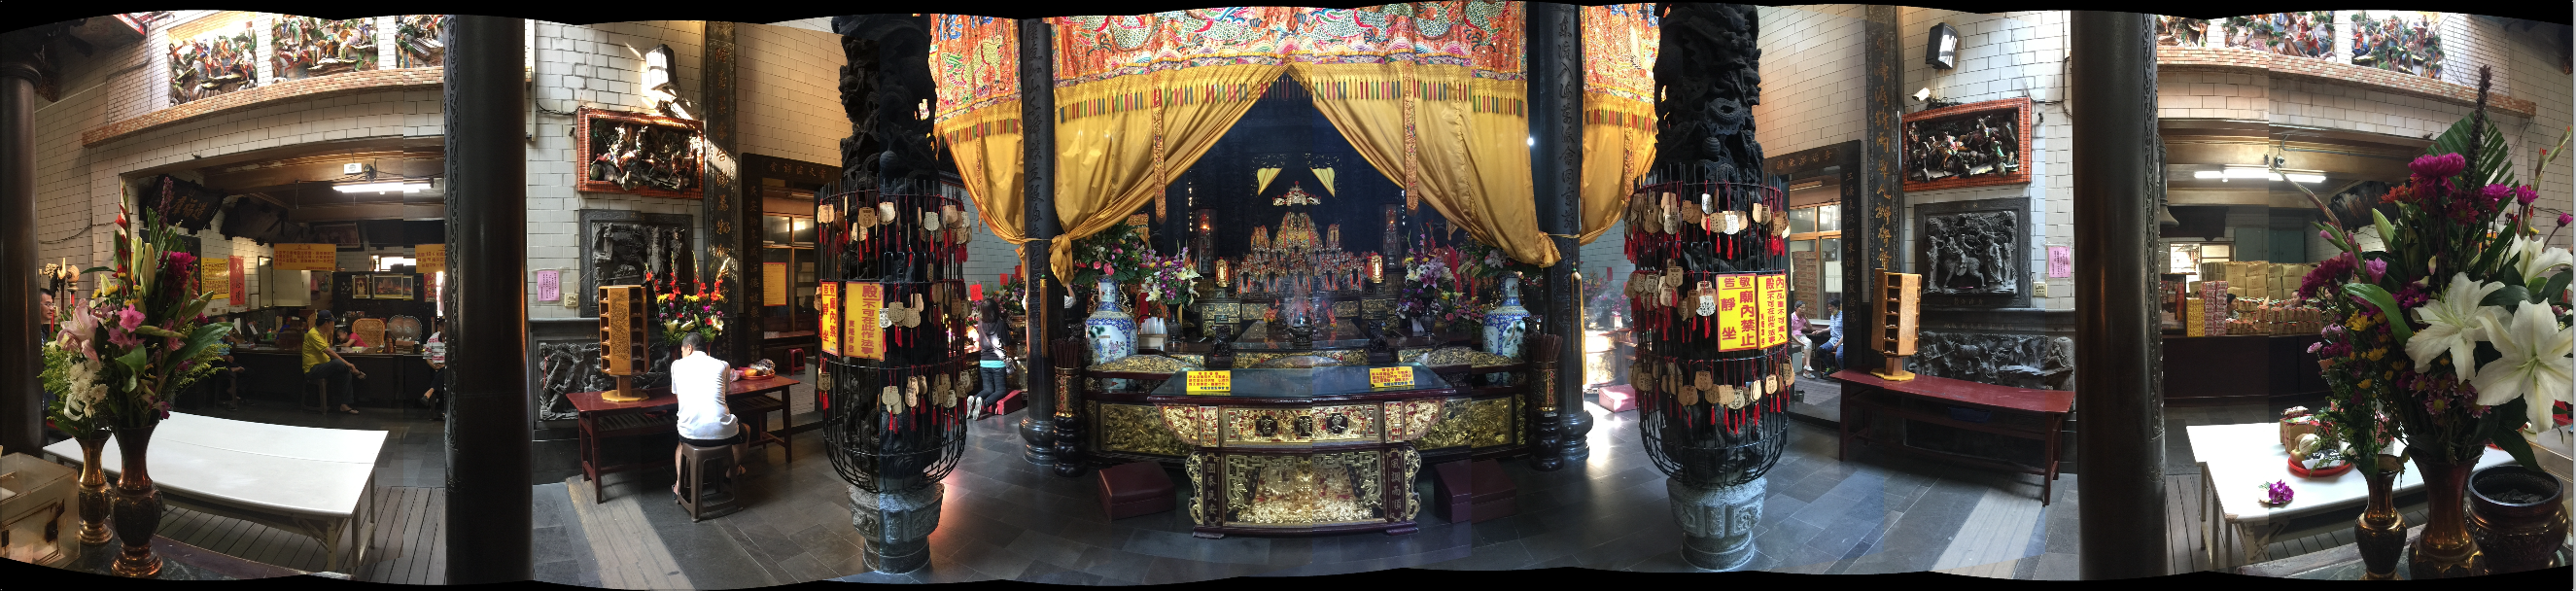
\includegraphics[width=\textwidth]{./figs/direct.png}}
  \caption{\textbf{Artifacts using direct blending}}
  \label{fig:direct}
\end{figure*}

\subsection{Alpha Blending}
This is almost as simple as direct blending, and it works better when the brightness
between images aren't consistent since it blends the overlapping region with gradient
like weight so that instead of an abrupt border line, you get a gradual transition.

The following artifacts uses alpha blending. Observing the following results, it
can be seen that if the camera is well-calibrated and alignment is done perfectly,
as is the case for the ``parrington'' dataset, alpha blending performs relatively
well. However, if the sequence of images are not carefully taken and there exists
misalignment, using alpha blending is going to blur up the overlapping region,
resulting in very poor panorama.

\begin{figure*}[h]
  \centering
  \subfloat[Parrington using alpha blending] {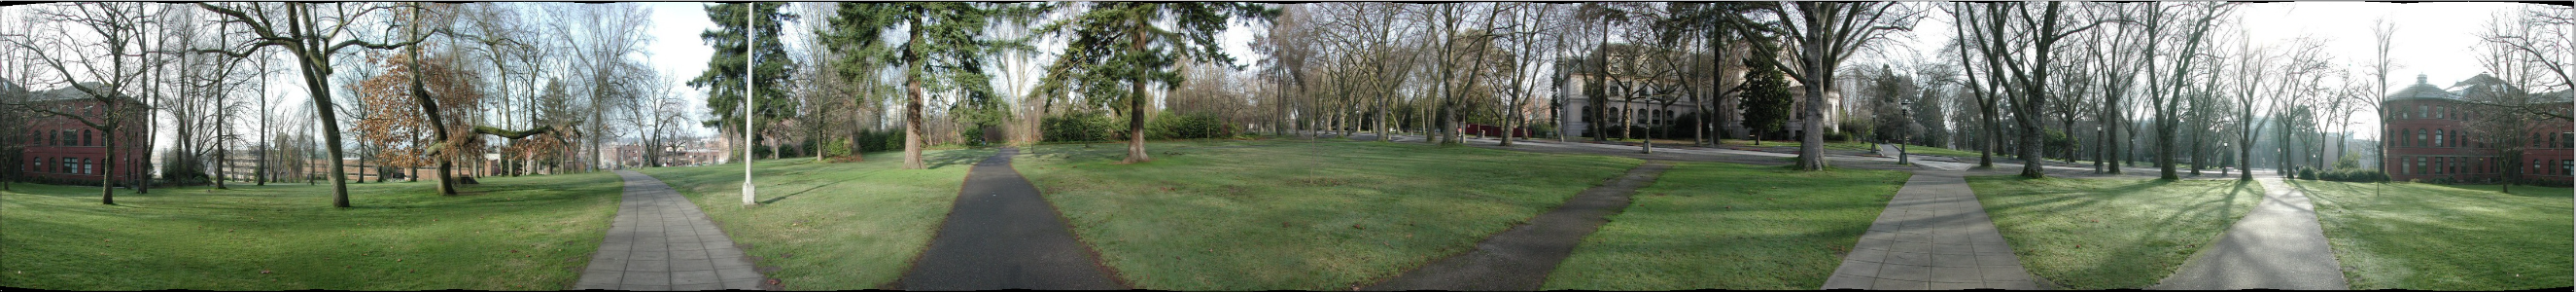
\includegraphics[width=\textwidth]{./figs/alpha1.png}}
  \hfill
  \subfloat[Temple using alpha blending] {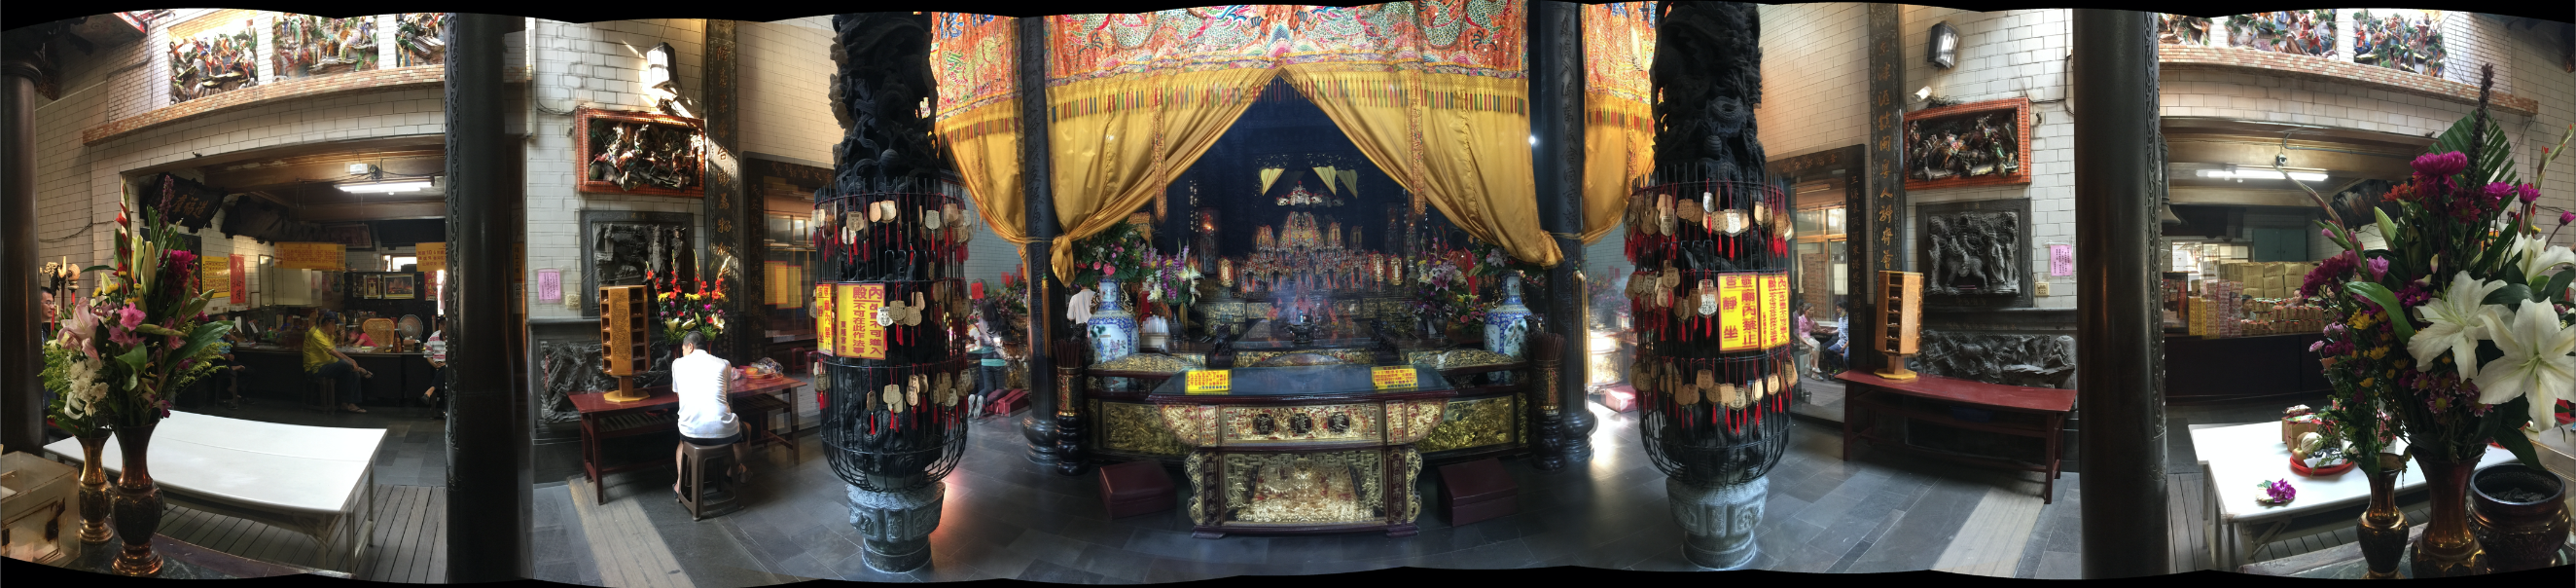
\includegraphics[width=\textwidth]{./figs/alpha2.png}}
  \caption{\textbf{Artifacts using alpha blending}}
  \label{fig:alpha}
\end{figure*}

\subsection{Poisson Blending}
This is the most complicated method that we've implemented. It was proposed by Perez
et al. \cite{Perez:2003:PIE:1201775.882269}. This involves solving a Poisson
partial differential equation with Dirichlet conditions, which is then discretized
to solving a symmetric, positive definite linear system. And since the system is
sparse, we implemented the iterative version of conjugate gradient method ourselves.
The main idea of this method is to add image one by one and optimize the difference
between the gradient of the resulting image and that of the original image under given
initial conditions. Please refer to our code for more implementation details.

The following shows some snapshot during the process of poisson blending.
Though judging from the result, poisson blending does a great job at creating
seamless image stitching. There are still two major fallbacks.

\begin{enumerate}
  \item {\bf It's time-consuming.} Though we have already used the conjugate
    gradient method which converges relatively fast compared to many other
    numerical methods, it's still very time-consuming when the resolution of your
    images increases.

    \clearpage
\begin{figure*}[h]
  \centering
  \subfloat[Initial condition] {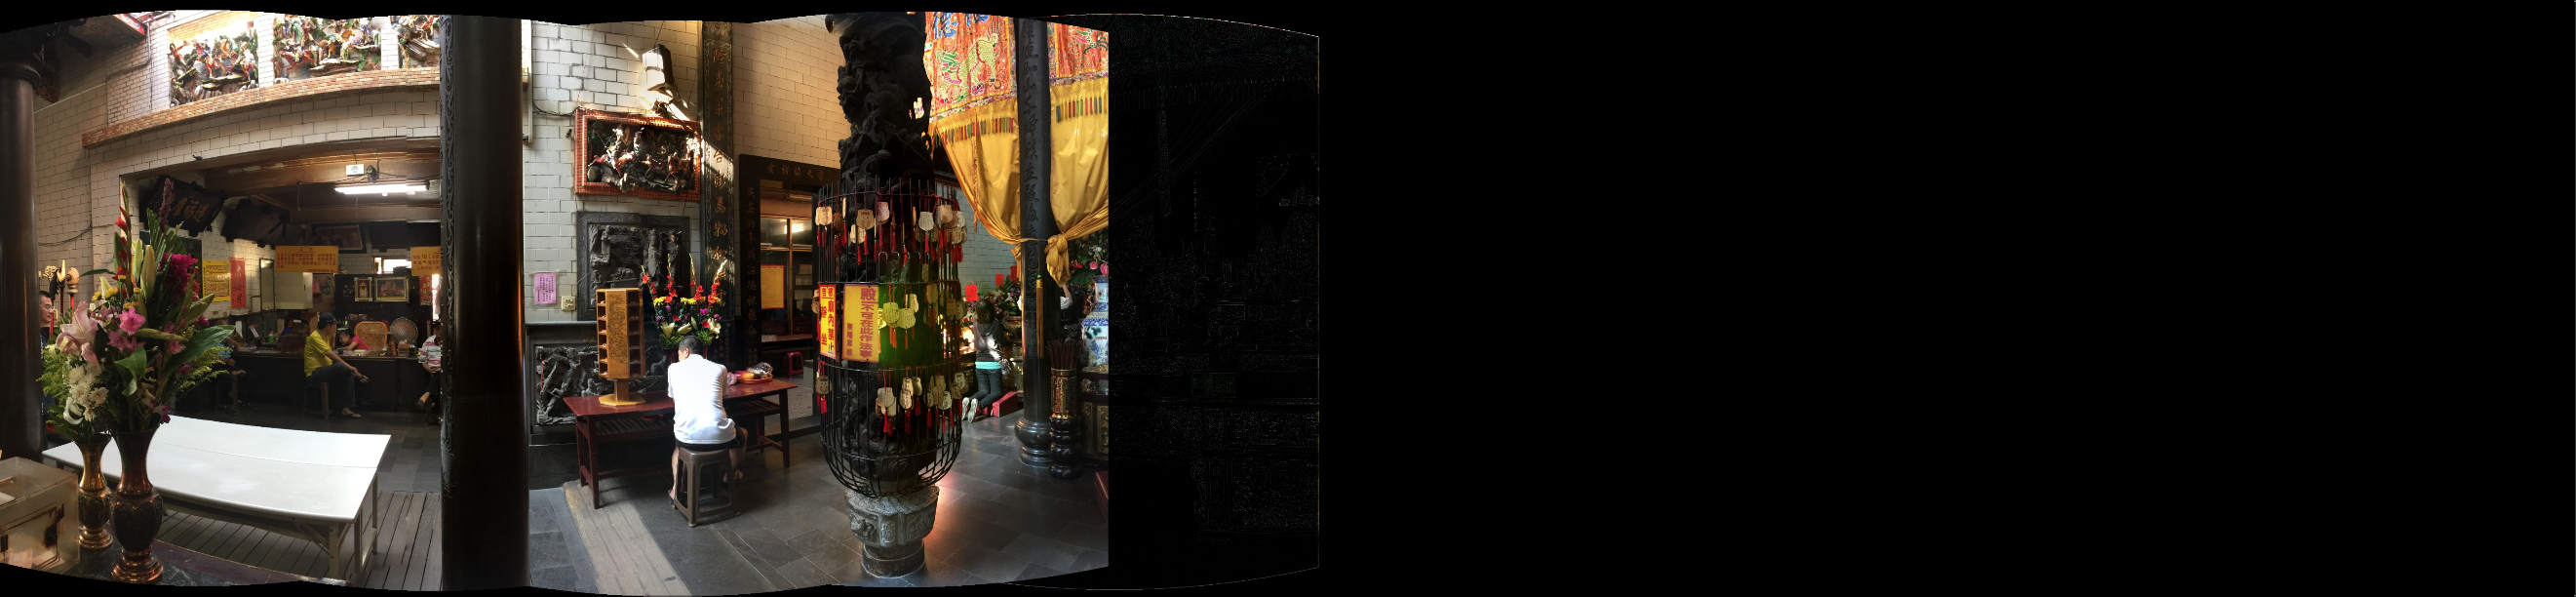
\includegraphics[width=\textwidth]{./figs/poisson2.png}}
  \hfill
  \subfloat[150 iterations] {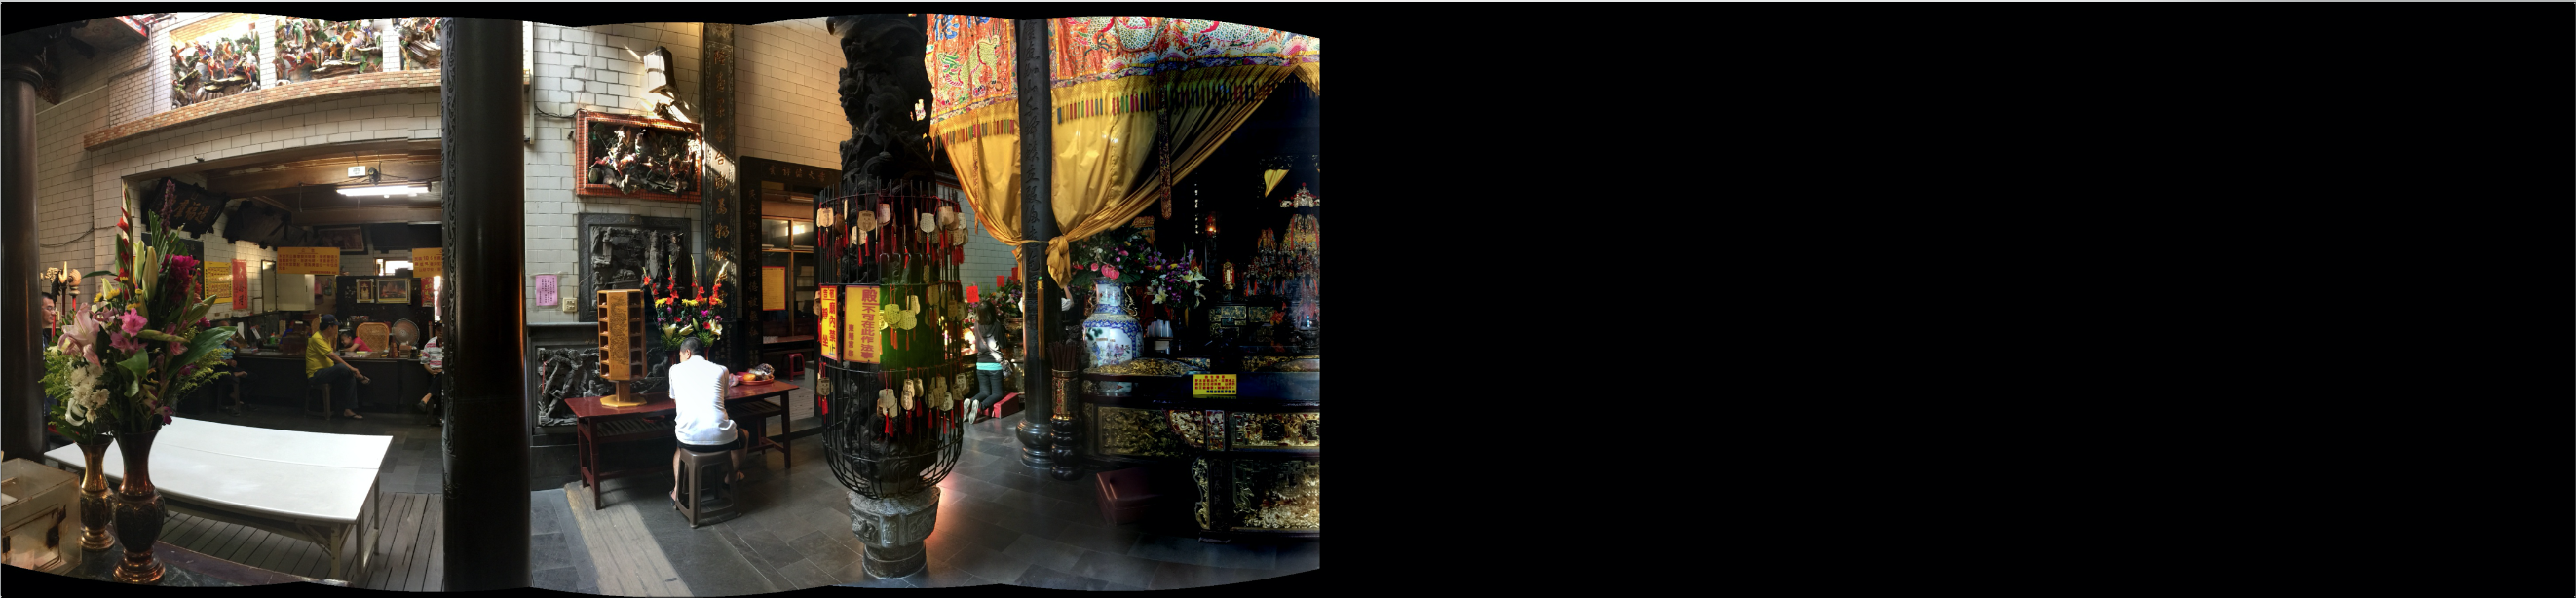
\includegraphics[width=\textwidth]{./figs/poisson3.png}}
  \hfill
  \subfloat[300 iterations] {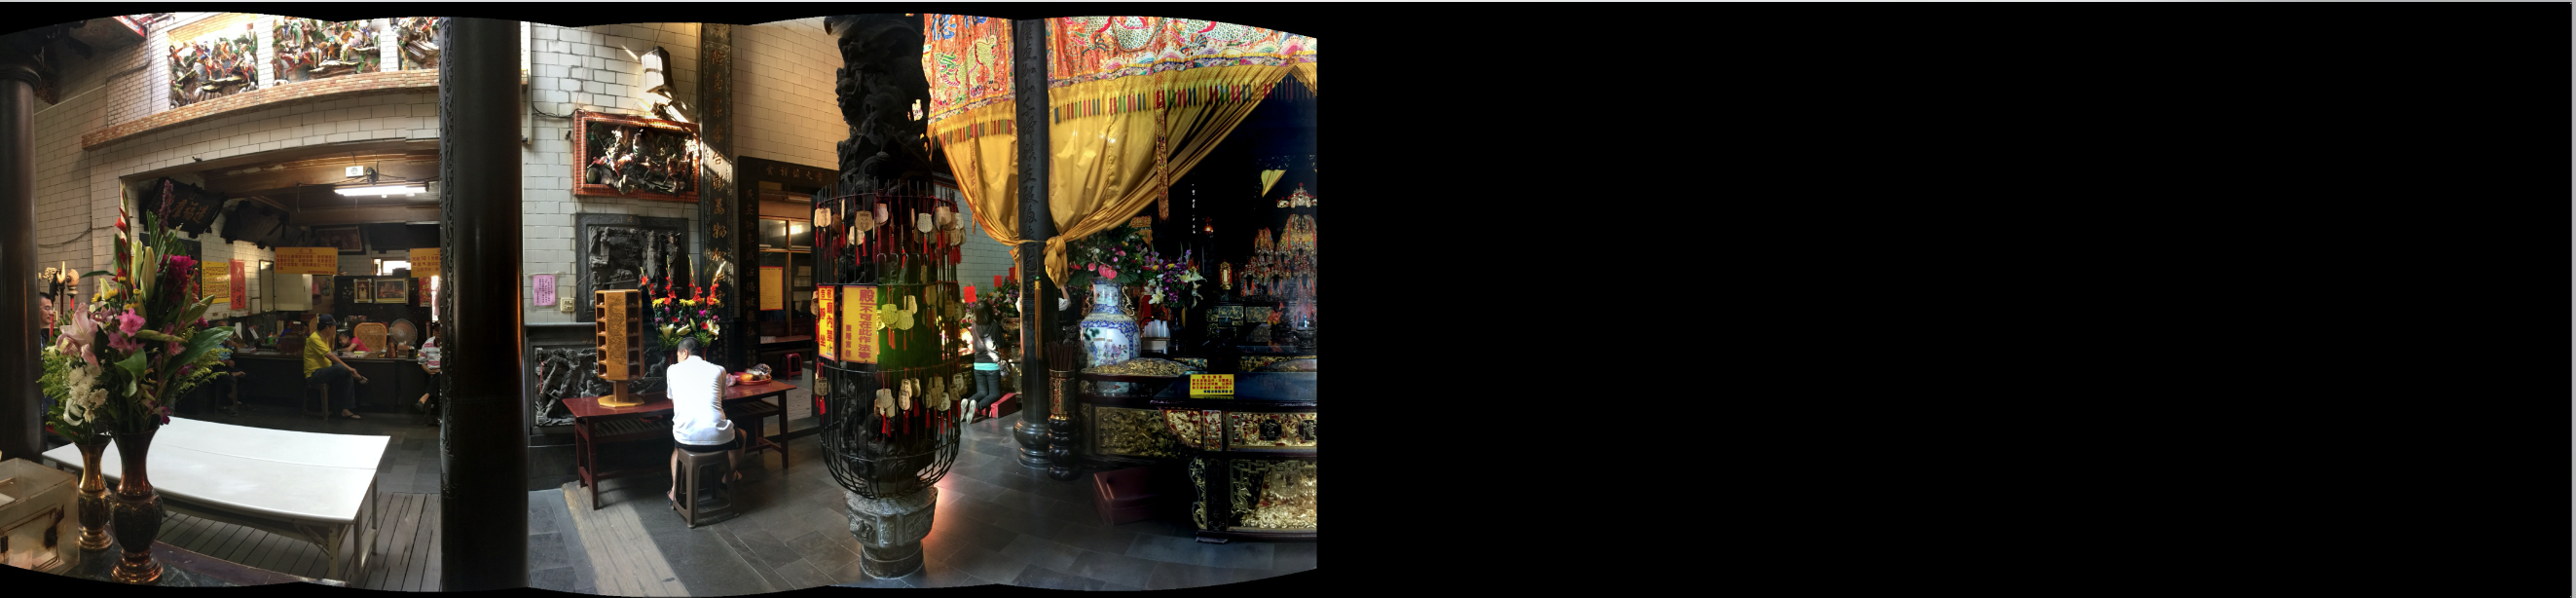
\includegraphics[width=\textwidth]{./figs/poisson4.png}}
  \hfill
  \subfloat[450 iterations] {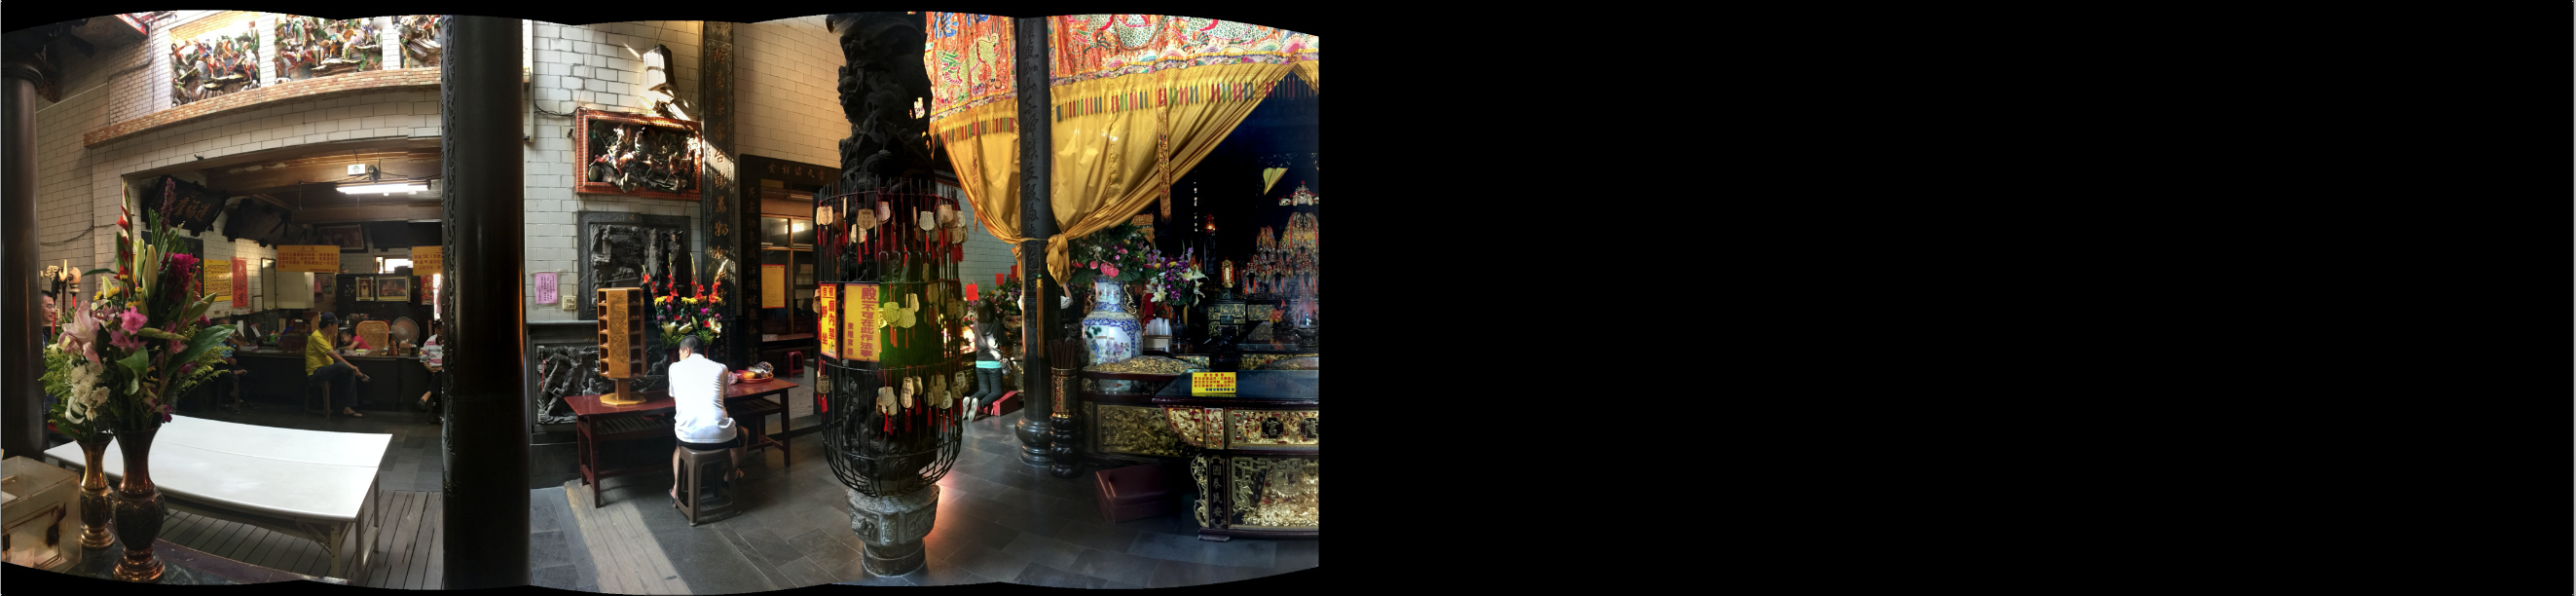
\includegraphics[width=\textwidth]{./figs/poisson5.png}}
  \hfill
  \subfloat[750 iterations] {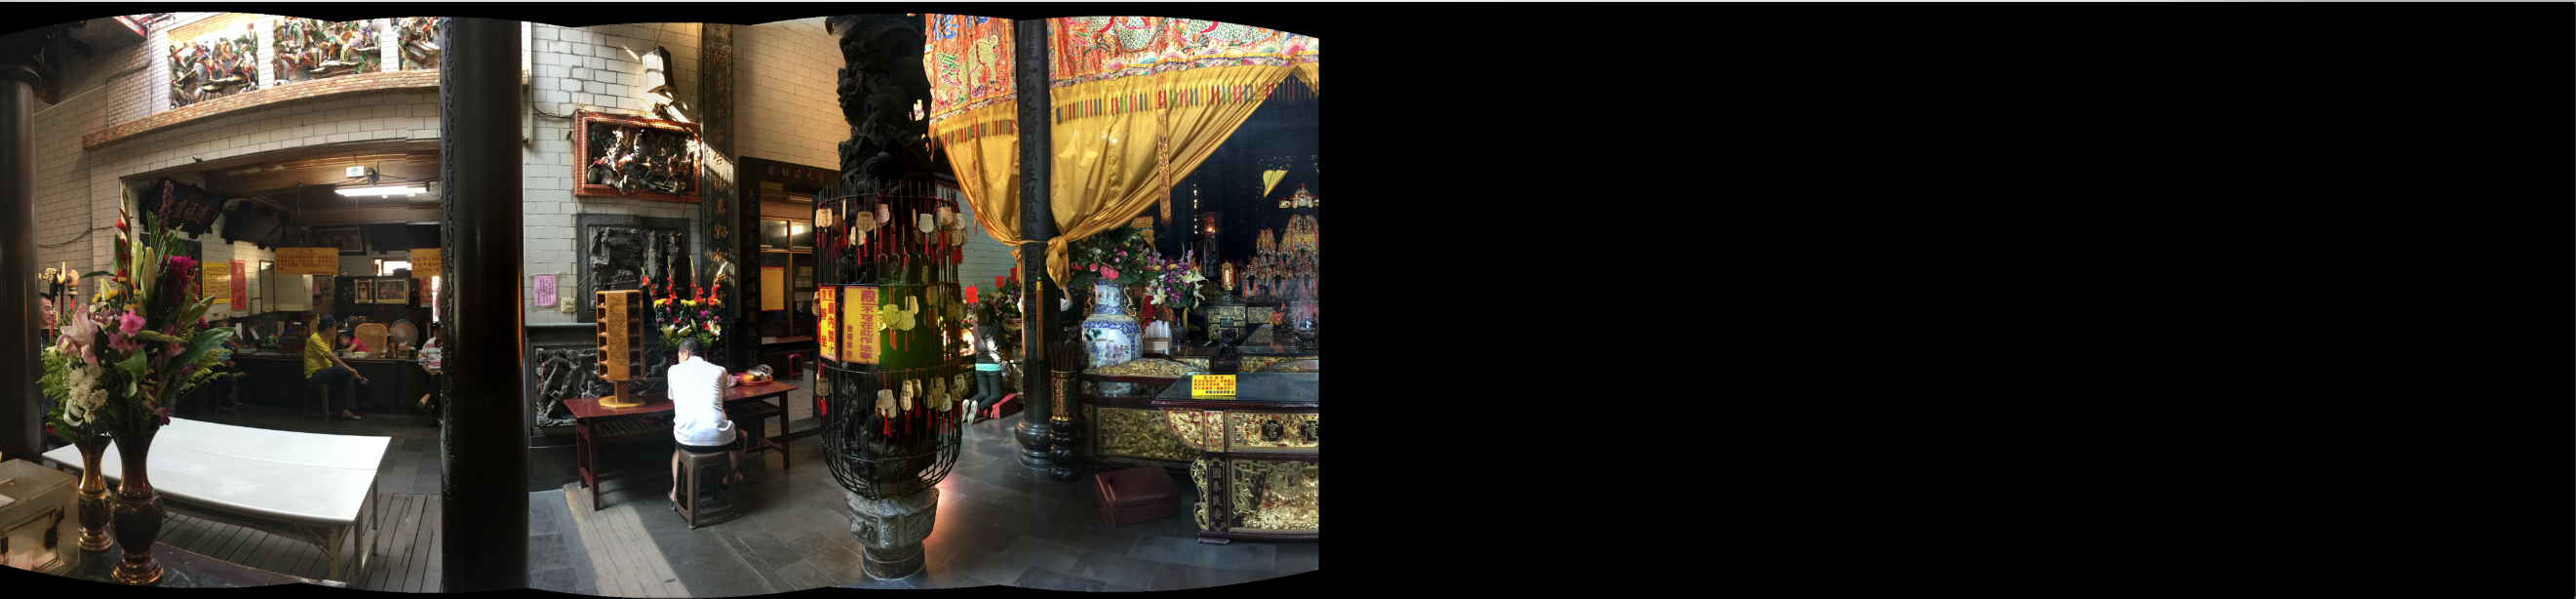
\includegraphics[width=\textwidth]{./figs/poisson7.png}}
  \caption{\textbf{Process of Poisson Blending}}
  \label{fig:poisson}
\end{figure*}
    \clearpage
  \item {\bf Doesn't handle misalignment.} Though the method tries to optimize
    the minimum difference between the gradients, it can barely help you in any way
    when your images are not perfectly aligned. Take a look at the artifacts in
    the next section and you can definitely spot some flaws.
\end{enumerate}

\section{Our Program}
The main program are written in C++ along with OpenCV. The executable submitted is built on macOS 10.12 with clang, if you can't execute it on your platform, build it from source as long as CMake ($\ge 2.8$) ,OpenCV, and g++ are available. For more details on executing our program, refer to the README file provided.

\section{Artifacts}
\begin{figure*}[h]
  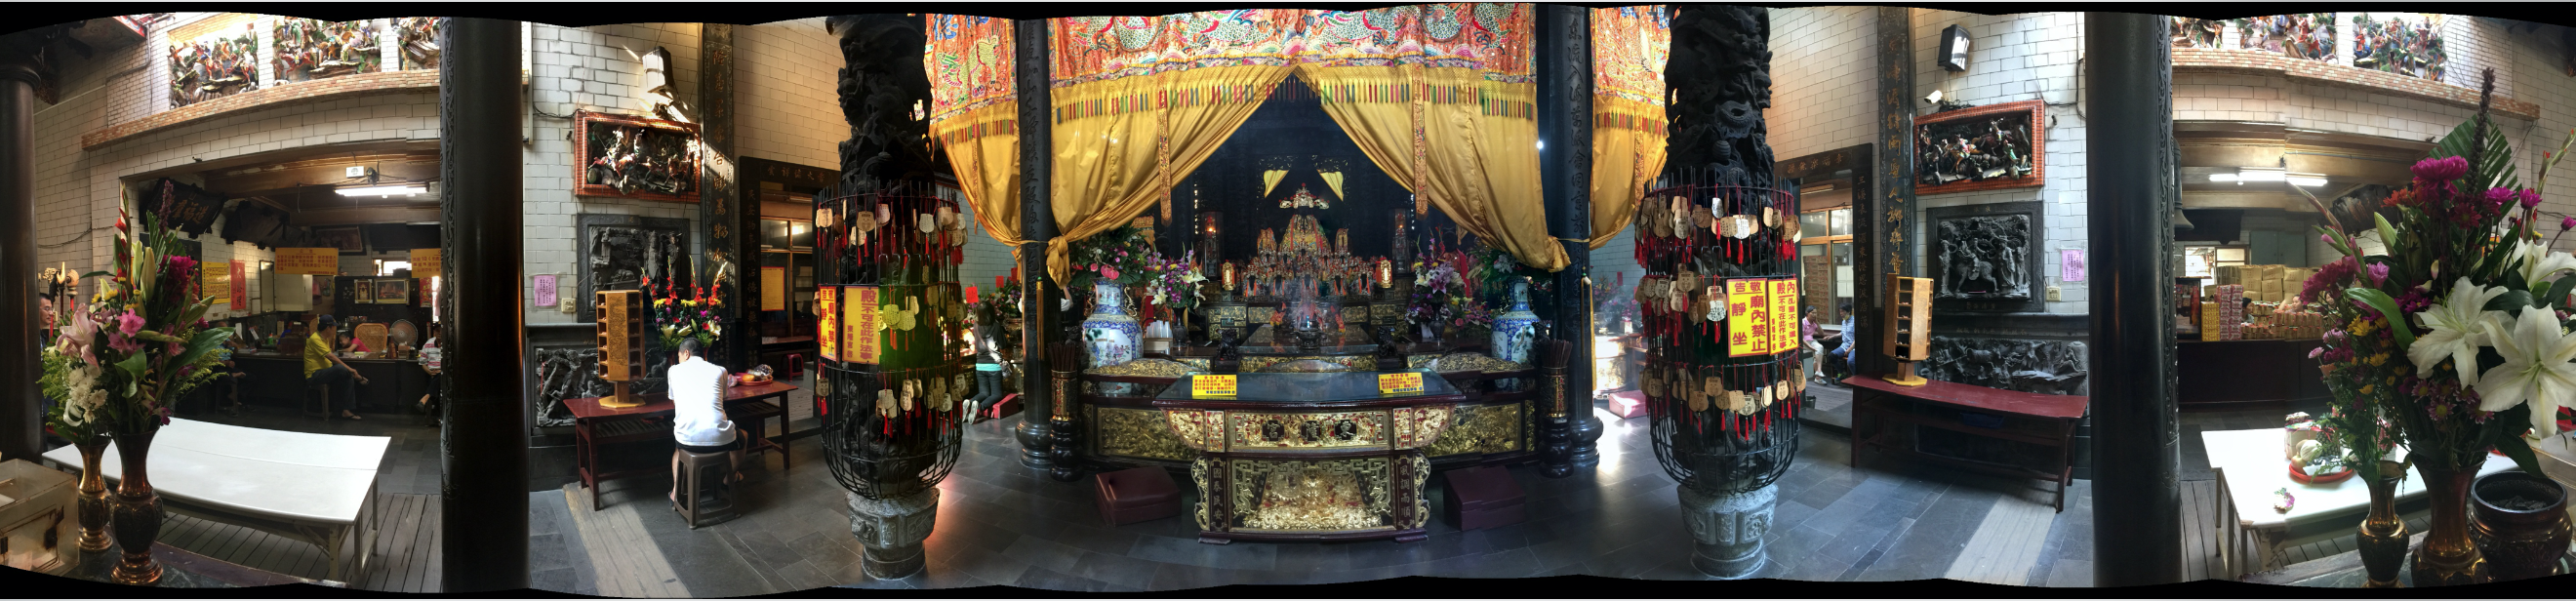
\includegraphics[width=\textwidth]{./figs/poisson8.png}
  \caption{\bf Temple, iPhone 6s, poisson blending}
\end{figure*}
\begin{figure*}[h]
  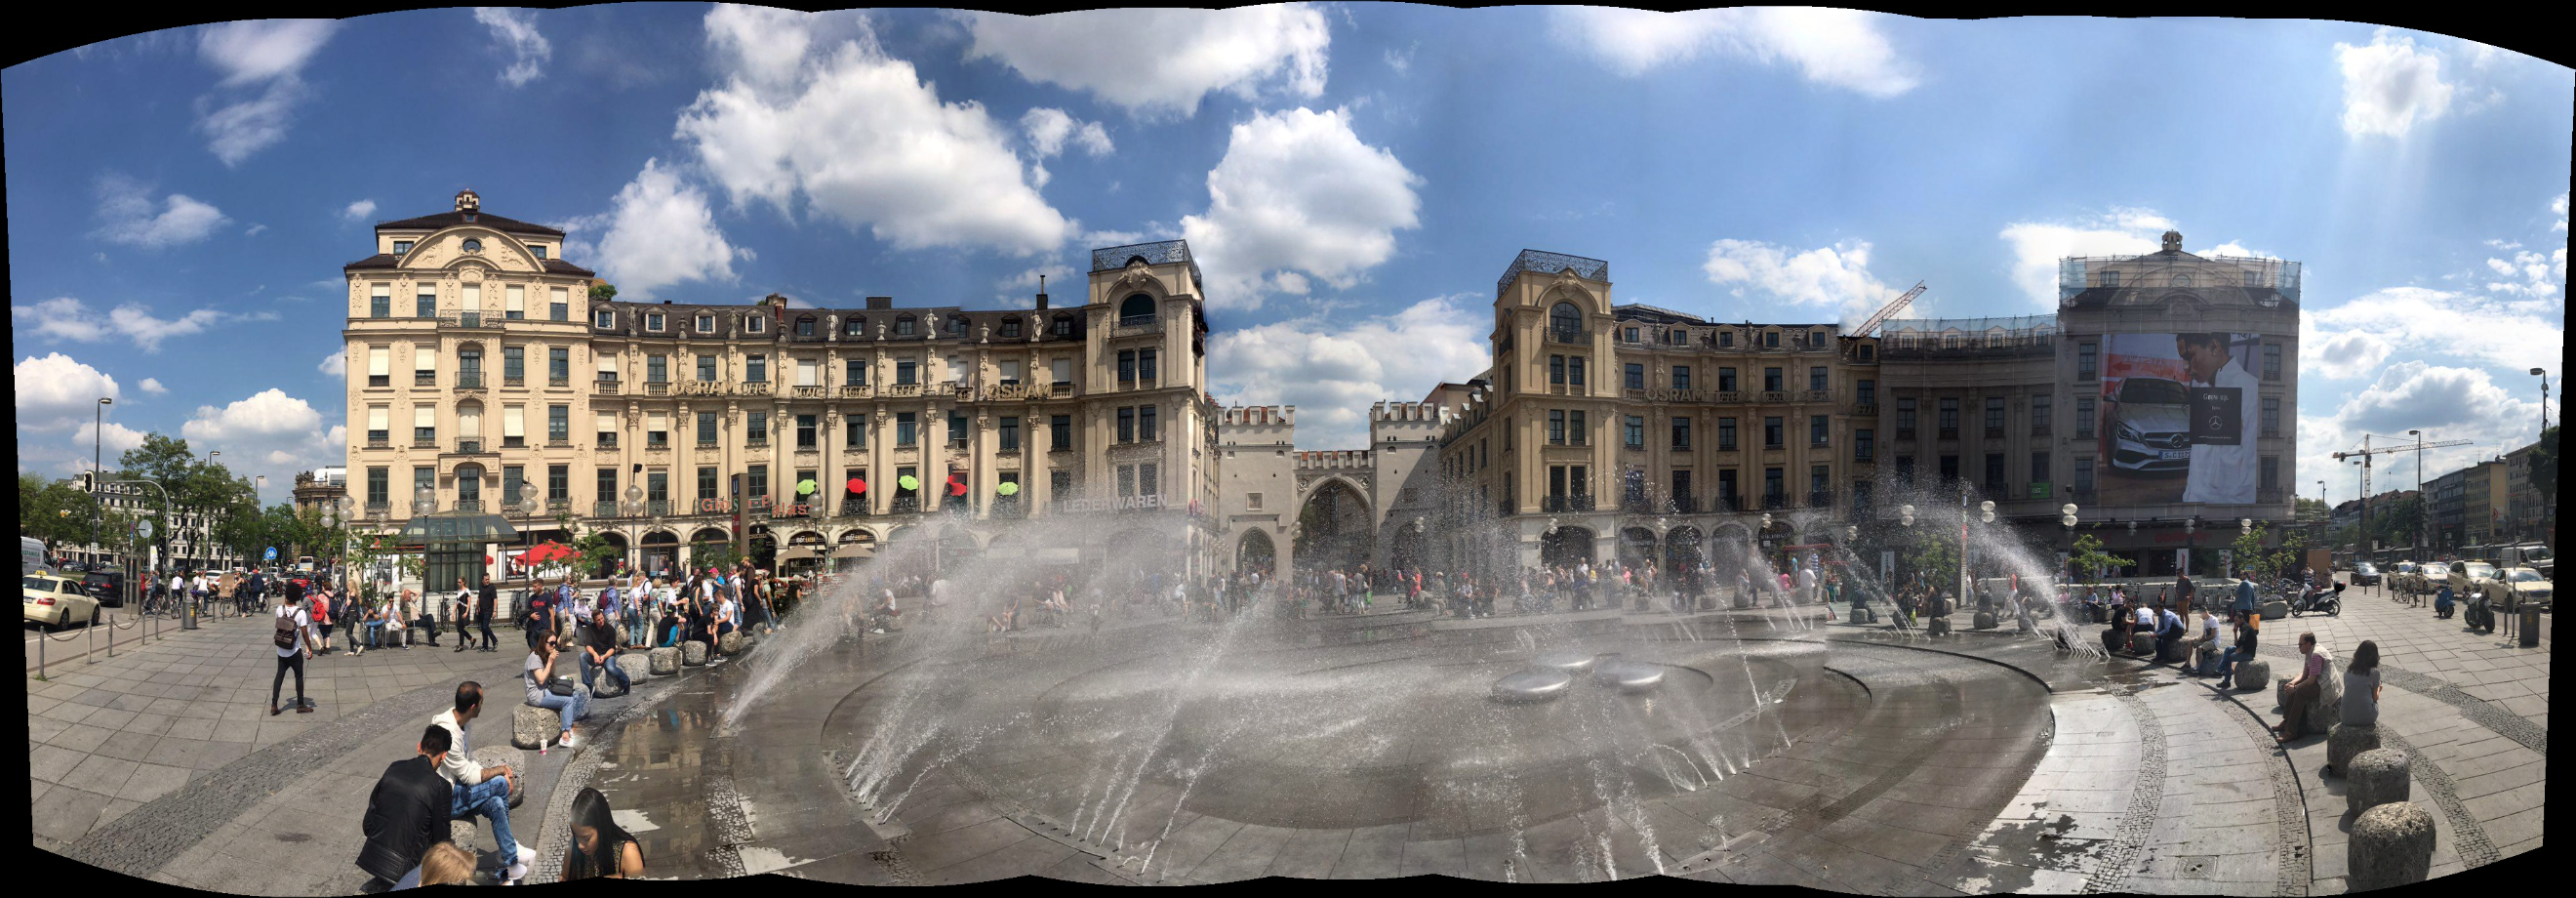
\includegraphics[width=\textwidth]{./figs/poisson9.png}
  \caption{\bf Fountain, iPhone 6s, poisson blending}
\end{figure*}

\bibliographystyle{unsrt}
\bibliography{citations.bib}

\end{document}
